\documentclass[titlepage]{jsarticle}
\usepackage[dvipdfmx]{graphicx}
\usepackage{listings}
\usepackage{h31ec-exp}
\lstset{
  basicstyle={\ttfamily},
  identifierstyle={\small},
  commentstyle={\smallitshape},
  keywordstyle={\small\bfseries},
  ndkeywordstyle={\small},
  stringstyle={\small\ttfamily},
  frame={tb},
  breaklines=true,
  columns=[l]{fullflexible},
  numbers=left,
  xrightmargin=0zw,
  xleftmargin=3zw,
  numberstyle={\scriptsize},
  stepnumber=1,
  numbersep=1zw,
  lineskip=-0.5ex
}
\renewcommand{\lstlistingname}{ソースコード}
\makeatletter
\newcommand{\figcaption}[1]{\def\@captype{figure}\caption{#1}}
\newcommand{\tblcaption}[1]{\def\@captype{table}\caption{#1}}
\makeatother
\title{IoTシステム開発の基礎}
\grade{3年32番}
\author{平田 蓮}
\team{第4班}
\date{2019年11月19日}
\expdate{2019年11月6日, 11月11日, 11月18日}
\coauthor{
    4番  石橋那起 \\
    8番  小林歩夢 \\
    12番  小室弦太 \\
    15番  佐藤貴幸 \\
    20番  関晋一朗 \\
    24番 高橋祐己哉 \\
    28番 外川諒太郎 \\
    36番  本多充稔
}

\begin{document}
\maketitle
\section{目的}
    本実験では, Raspberry Piを用いてLinux環境を構築し, その手順とともにIoT(Internet of Things)
    システム開発の基礎を習得する.

\section{実験手順}
    \subsection{Linux環境の構築}
        Raspberry Piでは内蔵されたストレージからではなく,
        microSDカードからOSを読み込んで起動する.
        そのため, Raspberry Piを使用するためにOSが入ったmicroSDカードを用意する
        必要がある. 今回はRaspberry Pi公式サポートOSであるRaspbianを使用する.

        以下に大まかな手順を示す.

        \begin{enumerate}
            \item OSファイルの準備
            \item Raspberry Piの起動, OSのインストール
            \item Raspbianの初期設定
        \end{enumerate}

        \subsubsection{OSファイルの準備}
            必要なOSファイルは, 校内サーバーからダウンロードをして使用する.

            \begin{enumerate}
                \item http://ftp.nagaoka-ct.ac.jp/pub/linux/raspbian
                    にアクセスしてNOOBS\_v3\_2\_0.zipダウンロードする
                    (このとき, デスクトップに保存しないと容量が足りないので気を付ける).
                \item microSDカードをPCに接続し, 解凍したファイルの中身を全てコピーする.
                \item デスクトップにあるzipファイルを削除する.
            \end{enumerate}

        \subsubsection{Raspberry Piの起動, OSのインストール}
            \begin{enumerate}
                \item もう一つのモニターからPCと周辺機器に接続しているケーブル類を外し,
                    今回の実験で使うものを代わりに接続する.
                \item Raspberry PiにmicroSDカード, HDMIケーブル, 周辺機器のケーブルを
                    接続する.
                \item Raspberry Piに電源ケーブルを接続し, 起動する.
                \item 画面に出る指示に従いインストールを進める.
            \end{enumerate}

        \subsubsection{Raspbianの初期設定}
            インストールが完了してRaspberry Piが起動したらLANケーブルをRaspberry Pi
            に接続し, 初期設定を進める.

            \begin{enumerate}
                \item プロキシの設定をする.
                
                    Raspberry Piでターミナルを開き, 以下の内容を/etc/apt/apt.confに
                    書き込む.

                    \verb|sudo vi /etc/apt/apt.conf|

                    \begin{lstlisting}[caption=apt.conf]
Acquire::http::proxy "http://st-proxy.st.nagaoka-ct.ac.jp:8080/";
Acquire::https::proxy "https://st-proxy.st.nagaoka-ct.ac.jp:8080/";
Acquire::ftp::proxy "ftp://st-proxy.st.nagaoka-ct.ac.jp:8080/";
                    \end{lstlisting}
                    
                    次に, /etc/profile.d/proxy.shに以下の内容を書き込む.

                    \verb|sudo vi /etc/profile.d/proxy.sh|

                    \begin{lstlisting}[caption=proxy.sh]
export HTTP_PROXY="http://st-proxy.st.nagaoka-ct.ac.jp:8080"
export HTTPS_PROXY="https://st-proxy.st.nagaoka-ct.ac.jp:8080"
export FTP_PROXY="ftp://st-proxy.st.nagaoka-ct.ac.jp:8080"
export NO_PROXY="127.0.0.1, localhost, 192.168.*.*"
                    \end{lstlisting}

                \item システムを更新する.
                    
                    プロキシの設定が終わったら, システムの更新を行う.

                    \verb|sudo apt-get update|

                    \verb|sudo apt-get upgrade|

                    終わったら, 再起動する.
            \end{enumerate}

    \subsection{IoTシステム作成}
        \subsubsection{センサー回路の作成とセンサー情報の読み取り} \label{sensor}
            今回は温湿度気圧センサーを使って部屋の温度, 湿度, 気圧を自動的に計測するシステムを作成する.

            \begin{enumerate}
                \item ブレッドボードを接続する.

                    Raspberry Piをシャットダウンし, GPIO-ブレッドボード接続ケーブルを用いて
                    Raspberry Piとブレッドボードを接続する.

                \item センサー回路を作成する.

                    BME-280センサモジュールをブレッドボードにセットし, 
                    資料を参考に配線を行う.

                    今回は$\mathrm I^2 \mathrm C$通信の設定を行う.

                    実際に作成した回路の配線図を図\ref{fig: haisen}に示す.

                    \begin{figure}[ht]
                        \centering
                        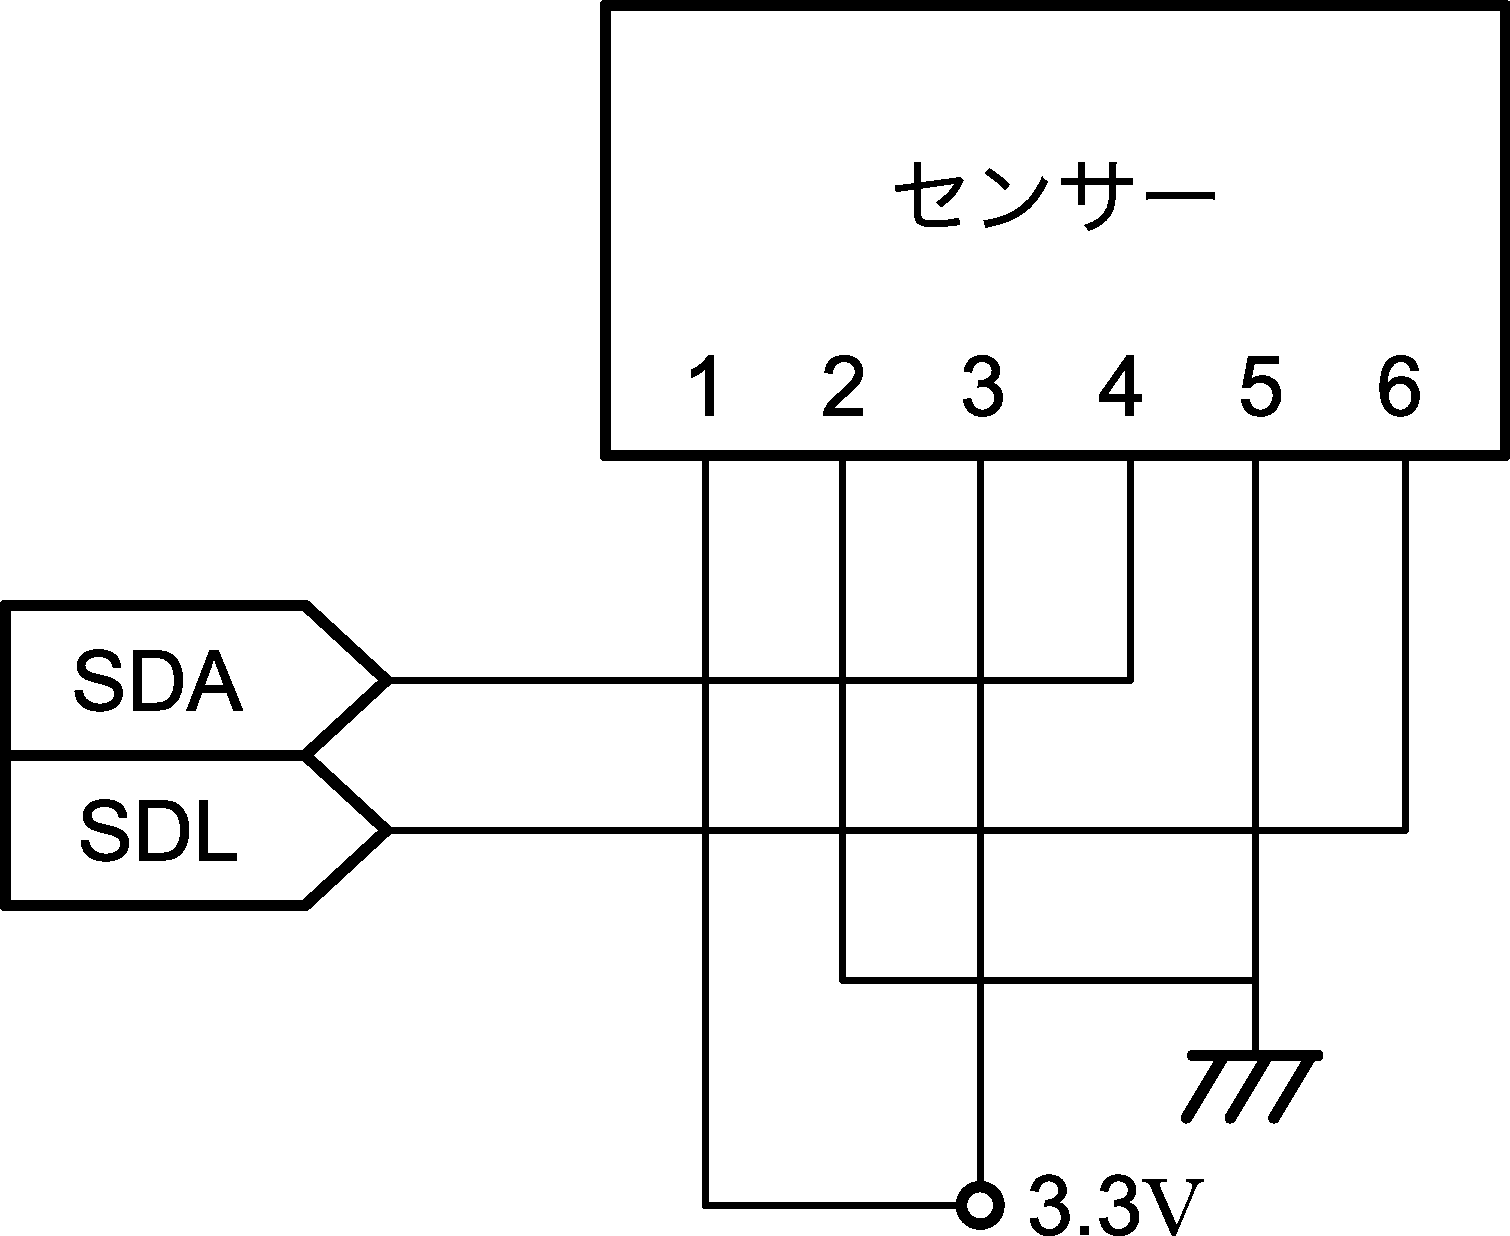
\includegraphics[width=10cm]{images/haisen.pdf}
                        \caption{配線図}
                        \label{fig: haisen}
                    \end{figure}

                \item $\mathrm I^2 \mathrm C$インターフェースを有効化する.
                
                    システムの設定メニューからRaspberry Piの設定を開き,
                    インターフェイスタブから, I2Cを有効にして保存する.

                \item https://github.com/SWITCHSCIENCE/BME280にアクセスして,
                    Python27フォルダからbme280\_sample.pyをダウンロードする.

                \item smbus2をインストールする.
                    
                    プログラムの実行に必要なsmbus2を以下のコマンドでインストールする.

                    \verb|sudo pip install --proxy="st-proxy.st.nagaoka-ct.ac.jp:8080" smbus2|

                \item 以下のコマンドでプログラムを実行する.
                
                    \verb|python bme280_sample.py|

                    実行に成功すると, 各情報が出力される.

            \end{enumerate}

        \subsubsection{Webシステムでの情報公開}
            今回は, apache2サーバーを使ってWebページを表示する.
            この節ではサーバーのインストールと設定を行う.

            \begin{enumerate}
                \item 以下のコマンドでapache2サーバーをインストール

                    \verb|sudo apt-get install apache2|

                \item 次に, CGIの設定を行う.
                
                    \verb|sudo ln -s /etc/apache2/mods-available/cgi.load /etc/apache2/mods-enabled/cgi.load|
                    
                    \verb|sudo chown pi /usr/lib/cgi-bin|

                    \verb|sudo service apache2 restart|

                \item 最後に, 以下のプログラムを/usr/lib/cgi-bin/に作成して動作確認をする.

                    \begin{lstlisting}[caption=test.cgi]
#!/usr/bin/python3
print('Content-Type: text/html')
print()
print('<html><body>')
print('<h1>Hello World!<h1>')
print('</body></html>')
                    \end{lstlisting}

                    http://localhost/cgi-bin/test.cgiにアクセスしてページが
                    表示されれば成功である.

            \end{enumerate}

    \subsection{温湿度, 気圧情報ページ作成}
        \subsubsection{サンプルコードの修正}
            \ref{sensor}節でダウンロードしたbme280\_sample.pyを/usr/lib/cgi-bin/にコピーして,
            Python3で動作するように以下の部分を書き換える.

            \verb|print <出力する文字列>| $\longrightarrow$ \verb|print(<出力する文字列>)|

        \subsubsection{CGIプログラムの作成}
            /usr/lib/cgi-bin/に以下のプログラムを作成する.
            
            \begin{lstlisting}[caption=tph-info.cgi]
#!/usr/bin/python3
from bme280_sample import readData()

print('Content-Type: text/html')
print()
print('<html><meta charset="utf-8"><body>')
print('<h3>Temperature, pressure and humidity information</h3>')
readData()
print('</body></html>')
            \end{lstlisting}

            このプログラムでは, htmlスクリプトを出力するとともに, 
            サンプルプログラムの関数を呼び出して, その関数で各情報を出力している.

            以下のコマンドで$\mathrm I^2 \mathrm C$デバイスファイルの属性を変更し,
            http://localhost/cgi-bin/tph-info.cgiで動作を確認する.

    \subsection{他のPCからページにアクセス} \label{ip}
        Raspberry Piで次のコマンドを実行してRaspberry Piのアドレスを取得する.
        (例: 192.168.50.149)

        \verb|ifconfig eth0|

        次に, Windowsで動作しているPCの方からhttp://\verb|<|\ref{ip}節で調べたアドレス\verb|>|
        /cgi-bin/tph-info.cgiにアクセスし, 動作を確認する.

\section{考察}
    今回はセンサーから情報を読み取る際にGitHubにあったサンプルコードを使用した.
    そのため, html出力をする際にサンプルコード内のprint文を改変する必要があった.

    今回はやらなかったが, そもそもサンプルコードの関数から湿温度, 気圧情報をそれぞれ
    返り値として取得することで, cgiファイル内のPythonスクリプトでオリジナルの操作を施しやすくなると考えた.

    使いやすいライブラリを作成することも大切であると改めて実感した.

\section{感想}
    今回のテーマは実験を行うのが初めてということで, 資料に間違いなどが見受けられた.
    しかし, エラーに直面しても, 自分で調べたり, 今まで学習してきた知識を活用することで
    修正することができた. この力は今後とても大切になってくると感じた.
    これからも学習を怠らないようにしたい.

\end{document}
